\section{Explicación del algoritmo}\label{implementacion}
Un sistema de captura de movimiento con las características necesarias para cumplir el objetivo de este proyecto debe implementar cuatro bloques generales: \emph{calibración}, \emph{detección de marcadores}, \emph{reconstrucción} y \emph{seguimiento}. En la Figura \ref{bloquesSist} se muestra un esquema del sistema a implementar, cada bloque verde indica la salida de una etapa siendo  a su vez la entrada del bloque siguiente.
%\vspace{-0.6cm}
\begin{figure}[ht!]
\centering
\hspace{-0.5cm}
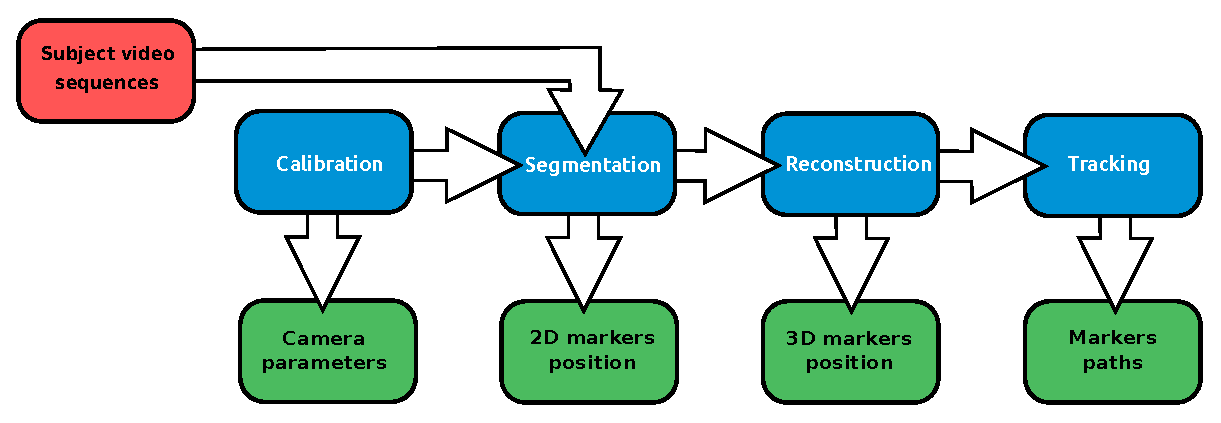
\includegraphics[scale=0.4]{imagenes/Sistema_completo/Diagrama_de_bloques.eps}
\caption{Diagrama de bloques del sistema completo.}
\label{bloquesSist}
\end{figure}
%\vspace{-0.7cm}
%Es importante destacar el hecho de poder separar el sistema en bloques independientes,

Es importante destacar la independencia entre bloques, permitiendo modificar u optimizar fácilmente el sistema en etapas futuras.
%. Esto asegura que el funcionamiento de uno de ellos no dependa del funcionamiento de otro. Por otro lado, da la posibilidad que en etapas futuras se pueda realizar el estudio de uno de los bloques de la Figura \ref{bloquesSist} individualmente y así poder modificarlo u optimizarlo sin afectar al resto.

